\hypertarget{ch:probability}{%
  \chapter{Probability -- Intuition and Paradoxes}
  \label{ch:probability}}

\chapterartfile{images/static/Black_Dice_PNG_Clip_Art-2653.png}
\hypertarget{Rintro}{The world is random and probability is a tool to quantify the randomness. It is the mathematical basis for all statistical reasoning. It helps us to determine how likely it is that we'll win a lottery, or the chances that our town will be hit by an earthquake in the next month.
However, probability theory can be confusing and even counter-intuitive in some cases. In this chapter we review basic concepts in probability, we show some examples in which our intuition may fail us (and even the best mathematician), and provide guidance how to avoid common errors in probabilistic thinking.}

\hypertarget{probability}{%
\section{Probability}\label{probability}}
\subsection{Basic Definitions}
%We will go through examples to see how probability helps interpret phenomena in real life and how probability may counter intuition. We begin by introducing some concepts:
We begin with some essential terminology and notations: 
\begin{itemize}
\item Experiment: a situation in which the outcome occurs randomly, e.g.,
  flipping a coin, rolling a dice, and picking a card from a deck.
\item Sample Space: the set of all possible outcomes in an experiment, e.g.,
  \{head, tail\}, \{1, 2, ..., 6\}, and \{all card faces\}.
\item Event: a subset of the sample space is called an event; an event
  occur if the outcome from an experiment belong to the event. For example, if
  you roll a dice, and you are interested in the result of having an even number,
  then the event is $E$=\{2, 4, 6\}.
\end{itemize}

The relationship between a sample space and an event can be illustrated using a
Venn diagram such as Figure~\ref{fig:probability-event} for rolling a die. The
sample space labeled as $S$ is represented by the outer rectangle that contains all the
six possible outcomes. The event $E$ of rolling an even number is represented
by the inner, rounded rectangle  that contains the numbers 2, 4, and 6.

\begin{figure}[htbp]
\centering
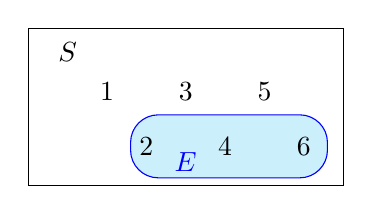
\begin{tikzpicture}
  \draw (-2, 2) rectangle (2, 0);
  \draw[rounded corners=10pt, fill = cyan!20, draw=blue] (-0.7,0.1) rectangle ++(2.5,0.8);
  \draw (-1.5, 1.7) node{$S$};
  \draw (-1, 1.2) node{1} (0, 1.2) node{3} (1, 1.2) node{5};
  \draw (-0.5, 0.5) node{2} (0.5, 0.5) node{4} (1.5, 0.5) node{6};
  \draw[text = blue] (0, 0.3) node{$E$};
\end{tikzpicture}
\caption{Sample space (the outcomes of a fair six-sided die) and event (rolling an even number) illustrated with Venn diagram. }
\label{fig:probability-event}
\end{figure}

\emph{Probability} is a number between zero and one which tells us how likely an event to occur. If we assume (for now) that the sample space is finite and each possible outcome in an experiment  has an equal chance to occur, then the probability of event $E$ is
  \begin{equation}
    P(E) =\frac{\text{size of } E}{\text{size of } S}.
  \end{equation}
  In the example depicted in Figure~\ref{fig:probability-event} the probability that we roll an even number when we use a fair die, is $P(even)=3/6=0.5$.
  
In the following chapters we will deal with infinite (even uncountable) sample spaces, and we will generalize the definition of $P(E)$ then.
  
 \begin{example}[Elevator waiting time]
  Mr. Smith works on the 13th floor of a 15 floor building. The only elevator in his building  moves continuously through floors 1, 2, . . . 14, 15, 14, . . . 2, 1, 2,  . . . , except that it stops on a floor on which the button has been
  pressed. Assume that time spent loading and unloading passengers is very small
  compared to the traveling time.  Mr.~Smith complains that at 5pm, when he
  wants to go home, the elevator almost always goes up when it stops on his
  floor. What is the explanation?
\end{example}

When Mr.~Smith gets to the elevator, it may be below the 13th floor or above
it. The elevator will go up if it is below the 13th floor and it will go
down if it is above the 13th floor. There are 12 floors below the 13th floor and
2 floors above it, so the probability that the elevator is below the 13th floor
is $12/14\approx0.86>0.5$. Thus no matter when Mr. Smith wants to go home, it is
more likely that the elevator is going up.

We can simulate this situation:

\showCode{R}{Code/probability-elevator.R}
\runR{Code/probability-elevator.R}{elevator}{}
Running the above code gives:
\includeOutput{elevator}

  
\hypertarget{conditional}{%
\subsection{Conditional Probability}\label{conditional}}

When there are two events $A$ and $B$ under consideration, knowing that $A$ has occurred may change the probability for $B$ to occur. For example, suppose that someone rolls a die behind a curtain and tells us only that the number is less than or equal to 3. What is the probability that it is an even number? Given that we got 1, 2, or 3, the only possibility that it is even is if the number is 2. The \emph{unconditional} probability of getting an even number in a roll of a die is 1/2, but because of the information that provided to us, we conclude that the \emph{conditional} probability is 1/3. 
Using mathematical notation, we write  $P(B\mid A)=1/3$ which stands for ``conditional on $A$=the number is less than or equal to 3, the probability of $B$=the number is even, is 1/3''. 

Once again, it is helpful to visualize such things using a Venn diagram. In Figure~\ref{fig:probability-conditional}, the sample space $S$ consists of the six possible outcomes and the two events are depicted as a circle (event $A$) and as a rounded rectangle ($B$). To say that we condition on $A$ means that we restrict our view and look only at outcomes that could occur if we are told that $A$ has occurred. In other words, our sample space becomes $A$, instead of the whole set, $S$.

\begin{figure}[htbp]
\centering
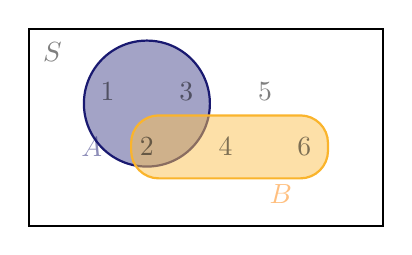
\begin{tikzpicture}[thick,fill opacity=0.5]
  \draw (-2, 2) rectangle (2.5, -0.5);
\draw[fill=MidnightBlue!80, draw=MidnightBlue] (-0.5, 1.05) circle (0.8);
  \draw[rounded corners=10pt, fill = Dandelion!80, draw=Dandelion] (-0.7,0.1) rectangle ++(2.5,0.8);
  \draw (-1.7, 1.7) node{$S$};
  \draw (-1, 1.2) node{1} (0, 1.2) node{3} (1, 1.2) node{5};
  \draw (-0.5, 0.5) node{2} (0.5, 0.5) node{4} (1.5, 0.5) node{6};
  \draw[text = orange] (1.2, -0.1) node{$B$};
  \draw[text = MidnightBlue] (-1.2, 0.5) node{$A$};
\end{tikzpicture}
\caption{Conditional probability -- given that we are told that a die gave a number less than or equal to 3 (event $A$), what is the probability that we got an even number ($B$)?}
\label{fig:probability-conditional}
\end{figure}

\bigskip
Can it be that we are told that some event $A$ has occurred, but this information tells us nothing about the probability of another event, $B$? Yes -- in this case we say that the two events are \emph{independent}, and we have
$$P(B\mid A) = P(B)\,.$$
In general, $P(B\mid A) \ge P(B)$.

\begin{example}[Two Children]
Consider the following two problems:
\begin{enumerate}
\item Mr. Jones has two children. The older child is a girl. What is the
  probability that both children are girls?
\item Mr. Smith has two children. At least one of them is a girl. What is the
  probability that both children are girls?
\end{enumerate}
\end{example}
In a family with two children there are four possible combinations of boy/girl in when we take into consideration their ages: \{Boy, Boy\},
\{Boy, Girl\}, \{Girl, Boy\}, \{Girl,Girl\}. Suppose that they all have the same probability to occur.

For the first question: the sample space for the given situation consists of only two events -- \{Girl, Boy\}, \{Girl,Girl\}; and only one of them corresponds to the event of having two girls. Thus the
probability of two girls is $\frac{1}{2}$. This question can also be solved this
way: Since the older child is a girl, the probability of two girls is the
probability that the younger child is a girl which is $\frac{1}{2}$.

For the second question, the sample space includes three possibilities: \{Boy, Girl\}, \{Girl, Boy\}, \{Girl,Girl\}. Thus the
probability of having two girls, given that at least one of them is a girl  is $\frac{1}{3}$.

If we simulate many families, we can find the numerical answer quite accurately.

\showCode{R}{Code/probability-TwoChildren.R}
\runR{Code/probability-TwoChildren.R}{TwoChildren}{}
Running the above code gives:
\includeOutput{TwoChildren}





\subsection{Bayes' Rule}\label{Bayes}
One of the most important results in probability and statistics looks deceivingly simple, but has deep consequences, as we will see in some of the subsequent examples. It is called Bayes' Rule, named after the reverend Thomas Bayes who discovered it in the 18th century. Consider two events, $A$ and $B$, such that $P(A)$ is greater than zero. Then
\begin{align}
  P(B\mid A) = \frac{P(A\mid B)P(B)}{P(A)},
\end{align}

 \begin{example}[Football or ballet?]
Jane has season tickets to the home games of her town's football team, which she attends  80\% of the time, and she also has season tickets to the town's ballet which she attends 20\% of the time. In 10\% of the weeks she attends both the weekly football game and the ballet. This is depicted in Figure~\ref{fig:bayes-rule}. 

If we see Jane in a game, what is the probability that we'll see her in the ballet in the same week?
Using Bayes' rule, $P(B\mid A) =0.5\times0.2/0.8=0.125$.

If we see her in the ballet, what is the probability that we will see her in the football game, as well?
With Bayes' rule we get $P(A\mid B) =0.125\times0.8/0.2=0.5$.

So, although Jane goes to  80\% of the football games, if she ends up going to the ballet then she is less likely to go to the game in the same week (50\%). 
\end{example}

\begin{figure}[htbp]
\centering
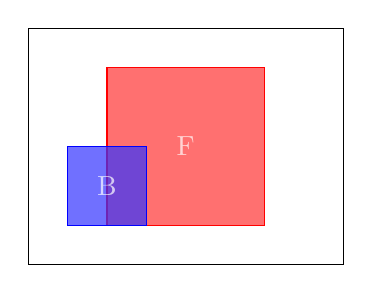
\begin{tikzpicture}[fill opacity=0.7]
  \draw (0,3) rectangle (4, 0);
  \draw[fill = red!80, draw=red] (1, 0.5) rectangle ++(2,2) node[midway,white]{F};
  \draw[fill = blue!80, draw=blue] (0.5,0.5) rectangle ++(1,1)  node[midway,white]{B};
\end{tikzpicture}
\caption{Bayes' rule. $F$ is the event that Jane attends the weekly football game, and $B$ is the events that she attends the weekly ballet.}
\label{fig:bayes-rule}
\end{figure}



\begin{example}[Bertrand's Box]
Bertrand's box paradox was first posed by Joseph Bertrand 1889. Here is the
question: There are three boxes, one contains two gold coins, one contains two
silver coins, and one contains a gold coin and a silver coin.
A box is selected at random and a coin is taken from that box at random. If the
coin is a gold coin, what is the probability that the other coin in that box is
also a gold coin.
\end{example}

This problem is about conditional probability. It is easy to find the
probability of getting a certain box, and it is easy to find the probability of
getting a gold coin if we know the box, as shown in
Figure~\ref{fig:probability-flow}. However, it is non-trivial to find the
difficulty of getting a certain box when we know the final coin. We see the six
possible outcomes in Figure~\ref{fig:probability-flow} are equally likely to
occur. Two outcomes of a gold coin are through the path of the box with two gold
coins and one outcome of a gold coin is through the path of the box with a gold
coin and a silver coin. Thus the answer to this problem is $\frac{2}{3}$.

\begin{figure}[H]
\centering
\resizebox{0.6\columnwidth}{!}{%
\begin{tikzpicture}[%scale=0.5,
  edge from parent/.style={draw,-latex},
    boxes/.style={star, draw=none, fill=red, drop shadow, text centered, anchor=north},
    state/.style={draw=none, fill=red, circle, drop shadow, text centered, anchor=north},
    leaf/.style={draw=none, fill=orange, ellipse, text centered, anchor=north},
    leafs/.style={draw=none, fill=gray, ellipse, text centered, anchor=north},
    level distance=0.9cm, growth parent anchor=south
]
\node [boxes] {Boxes} [->] [sibling distance=4cm]
child{ [sibling distance=2cm]
  node [state] {Gold, Gold}
  child{node [leaf] {Gold}
    edge from parent{node[left]{$\frac{1}{2}$}}
  }
  child{node [leaf] {Gold}
    edge from parent{node[right]{$\frac{1}{2}$}}
  }
  edge from parent{node[above right]{$\frac{1}{3}$}}
}
child{ [sibling distance=2cm]
  node [state] {Gold, Silver}
  child{node [leaf] {Gold}
    edge from parent{node[left]{$\frac{1}{2}$}}
  }
  child{node [leafs] {Silver}
    edge from parent{node[right]{$\frac{1}{2}$}}
  }
  edge from parent [dashed] {node[right]{$\frac{1}{3}$}}
}
child{ [sibling distance=2cm]
  node [state] {Silver, Silver}
  child{node [leafs] {Silver}
    edge from parent{node[left]{$\frac{1}{2}$}}
  }
  child{node [leafs] {Silver}
    edge from parent{node[right]{$\frac{1}{2}$}}
  }
  edge from parent [dashed] {node[above right]{$\frac{1}{3}$}}
};
\end{tikzpicture}
}
\caption{Probability flow for Bertrand's Box}
\label{fig:probability-flow}
\end{figure}

This problem can also be solved using the Bayesian formula. It says 
\begin{align}
  P(B\mid A) = \frac{P(A\mid B)P(B)}{P(A)},
\end{align}
where the conditional probability $P(B\mid A)$ is difficult to find but the
conditional probability $P(A\mid B)$ as well as the unconditional probabilities
are easy to find. If $A$ be the event of getting a gold coin and $B$ be the
event of getting a box with two gold coins, then $P(A)=\frac{1}{2}$,
$P(B)=\frac{1}{3}$, and $P(A|B)=1$. Now the probability of a box with two gold
coins given a final gold coin is 
\begin{align}
  % P(GG\mid G) = \frac{P(G\mid GG)P(GG)}{P(G)}
  P(B\mid A) = \frac{P(A\mid B)P(B)}{P(A)}
  = \frac{1\times\frac{1}{3}}{\frac{1}{2}}
  =\frac{2}{3}.
\end{align}

Both of the aforementioned two approaches give us the correct answer. However,
we don't have to go through the counting or reasoning. If we can simulate the
game, we can find the result pretty accurately. The following code simulate the 
game and approximate the probability numerically.

\showCode{R}{Code/probability-BertrandBox.R}
\runR{Code/probability-BertrandBox.R}{BertrandBox}{}
Running the above code gives:
\includeOutput{BertrandBox}

\section{When Intuition May Fail}
Probability-based logic may be confusing and even counter-intuitive in some cases. In this section, we show such cases, some of which have confused some of the brightest people. The purpose of introducing these examples is to show how they may occur in everyday situations, and how to deal with them correctly.

\hypertarget{Intransitive-Dice}{%
  \subsection{Intransitivity -- when $A>B$ and $B>C$ does not imply $A>C$}\label{Intransitive-Dice}}
Real numbers are transitive, meaning that if we know that $x>y$ and $y>z$ then $x>z$. However, probability of events are not always transitive. 
\begin{example}[Intransitive Dice]
We have three unusual dice:
\begin{itemize}
\item Die A has sides 2, 2, 4, 4, 9, 9.
\item Die B has sides 1, 1, 6, 6, 8, 8.
\item Die C has sides 3, 3, 5, 5, 7, 7.
\end{itemize}
\end{example}

To play a game you and your opponent choose two of the dice, say, A and B, and you get to choose which die you roll (and your opponent will roll the other.) The one who tolls a larger number wins. Which die do you want to choose?

Let's tabulate the possible results if dice A and B were chosen, and see which  die is preferred.
\begin{center}
  \begin{tabular}{cc|ccc}\hline
    &   & \multicolumn{3}{c}{B} \\
    % \cline{3-5}
    &   & 1                & 6                & 8                \\ \hline
    \multirow{3}{*}{A}
    & 2 & \color{red}$A>B$ & $A<B$            & $A<B$            \\
    & 4 & \color{red}$A>B$ & $A<B$            & $A<B$            \\
    & 9 & \color{red}$A>B$ & \color{red}$A>B$ & \color{red}$A>B$ \\\hline
  \end{tabular}
\end{center}

Since die A wins five out of the nine possible results and all possible results
occur with equal probability, we know that die A has a higher winning
probability ($\frac{5}{9}$) than die B. We should choose die A over die B.

Now suppose we choose dice B and C.
\begin{center}
  \begin{tabular}{cc|ccc}\hline
    &   & \multicolumn{3}{c}{B} \\
    % \cline{3-5}
    &   & 1                & 6                & 8                \\ \hline
    \multirow{3}{*}{C}
    & 3 & \color{red}$C>B$ & $C<B$            & $C<B$            \\
    & 5 & \color{red}$C>B$ & $C<B$            & $C<B$            \\
    & 7 & \color{red}$C>B$ & \color{red}$C>B$ & $C<B$ \\\hline
  \end{tabular}
\end{center}

We see that die B has a higher winning probability ($\frac{5}{9}$) than die C,
so we should choose die B over die C.

Since we should choose die A over die B, and choose die B over die C, does this
mean that we should choose die A over die C if these two dice are to be
selected? Surprisingly, the answer is NO. Here is the table of the possible
results.
\begin{center}
  \begin{tabular}{cc|ccc}\hline
    &   & \multicolumn{3}{c}{C} \\
    % \cline{3-5}
    &   & 3                & 5                & 7                \\ \hline
    \multirow{3}{*}{A}
    & 2 & $A<C$            & $A<C$            & $A<C$            \\
    & 4 & \color{red}$A>C$ & $A<C$            & $A<C$            \\
    & 9 & \color{red}$A>C$ & \color{red}$A>C$ & \color{red}$A>C$ \\\hline
  \end{tabular}
\end{center}
We should choose die C over die A!

Here is an experiment to simulate the intransitive dice.

\showCode{R}{Code/probability-IntransitiveDice.R}
Running this code gives the following:
\runR{Code/probability-IntransitiveDice.R}{IntransitiveDice}{}
\includeOutput{IntransitiveDice}


You are probably never going to encounter such dice, or play this game, but you may encounter a similar situation in real life when you have to choose among different people for a single position, or choose among similar products, based on preferences or ratings.
For example, suppose you want to purchase a new phone which is offered by three manufacturers, and there are six reviews for each phone. Note that the average ratings of all three options in our made-up example is the same. You may prefer phone A because it got the highest rating (twice). However, it also got two very low ratings, so choosing based on the maximum is risky. Option C has less variability in its ratings, but it didn't get a very high score from any reviewer. Furthermore, it may be that you have 60,000 reviews for each phone, and not just six. So, going systematically over the reviews is impractical, and you may decide that the best way to choose your phone is to use a randomized algorithm like the one in the dice example. That is, choose two of the options, and  then choose one random rating for each one, and select the one that give the highest score. This is a reasonable algorithm, but you have to be aware of the fact that when choices are made based on a probabilistic approach, ordering of options may not have the transitive property.



\hypertarget{birthday-problem}{%
  \subsection{Rare Events Still Happen}\label{birthday-problem}}

\begin{example}[Birthday Problem]
You go on a long trip on your birthday and take a bus. There are 23 people on the bus, and to make the ride more fun you ask all the other passengers for their birth date (month and day, not year) and see if you can celebrate together. How likely it is that someone on the bus shares your birthday?

The chance that a random person has the same birthday as yours is $1/365\approx0.0027$, so it may seem pretty unlikely, but with 23 people on the bus it turns out the the probability that at least one of them shares your birthday is much higher ($\approx0.061$.) In you took a plane with 253 passengers the probability that at least one of them shares your birthday is 0.5.

We will also answer the following question: what is the probability that on the bus/plane there are at least two people who share a birthday (even if it's not the same as yours)?
\end{example}

Let's use simulation to answer these questions.

\showCode{R}{Code/probability-birthday.R}
\runR{Code/probability-birthday.R}{birthday}{}
Running the above code gives results which are very close to the number we stated above, as predicted by probability. That is, if there are 23 people on the bus the probability that some people
share the same birthday is \inlnR{```cat(prob.p23[1])```} and the probability
that at least one person's birthday is the same as yours is
\inlnR{```cat(prob.p23[2])```}. If there are 253 people on the plane, the two
probabilities are \inlnR{```cat(prob.p253[1])```} and \inlnR{```cat(prob.p253[2])```}, respectively. 

This is an example that shows that rare events can occur quite often, if we have a large enough sample.
This is particularly important in trials, where DNA match is often used as evidence that a defendant has committed a crime. The chance that a DNA sample from a crime scene matches a random person is extremely low, but not zero. With nine billion people in the world, the probability that at least one other person's DNA (other than the true offender) will match the DNA sample from the scene is not negligible.

\textcolor{red}{Exercise}
Adapt the previous code by changing $N$ and $n$, to check the probability that a 1 in a billion event will be observed if you run the experiment with 1 million people.

\subsection{Predictions}
The following example is one of the earliest questions in probability, when the field was mostly of interest among gamblers (who were also prominent mathematicians).

\begin{example}[Fair Division]
Tom and Jerry each put 30 dollar in a jackpot to start a tennis match. They are equally good players, and have equal chance to win a match. They decide that the first one to win three matches will win the \$60. 
Now, Tom has won twice and Jerry has won once, but the matches took a long time and they had to go back home before a winner was declared. How should they split the 60 dollars, given the current position (Tom leading 2-1)?
\end{example}

It seems Tom has won twice and Jerry has won once so the 60 dollars should be
split as $40:20$. However, these are not proportional to their probabilities of
winning. They need at most another two games to know the final winner. Here are
the four possible winners of the next two games: \{Tom, Tom\}, \{Tom, Jerry\},
\{Jerry, Tom\}, \{Jerry, Jerry\}. In the first three possible outcome Tom ends up with 3 wins, and therefore would get the \$60, and only the fourth outcome leads to Jerry being the first to reach three wins.
So the probabilities that Tom and Jerry would be
the final winner are $\frac{3}{4}$ and $\frac{1}{4}$, respectively, and the fair
division should be $45:15$.

Let's use simulation to solve this problem.

\showCode{R}{Code/probability-FairDivision.R}
\runR{Code/probability-FairDivision.R}{FairDivision}{}
Running the above code gives:
\includeOutput{FairDivision}

The takeaway from this example is that it is not sufficient to know what has happened in the past in order to make accurate predictions. It is also necessary to know the `horizon' of the experiment (how much longer the experiment can run.) The same logic would apply if the winning probabilities in each match are not equal, and when the horizon is farther (more matches are needed in order to declare the winner.)

% real life example?



\hypertarget{Monty-Hall-problem}{%
\subsection{Jumping Probabilities}\label{Monty-Hall-problem}}

\begin{example}[Monty Hall Problem]
Suppose you're on a game show, and you're given the choice of three doors:
Behind one door is a car; behind the others, goats. Whichever door you pick, you get what's behind it.
You pick a door, say No. 1, and the host, who knows what's behind the doors, opens another door, say No. 3,
which has a goat. He then says to you, ``Do you want to pick door No. 2?'' Is it
to your advantage to switch your choice?
\end{example}

This famous example has confused many smart people. It is also about conditional
probability and can be solved by using the Bayesian formula. However, setting up
the conditional and unconditional probabilities for this problem is
complicated. Some people did not believe the result answer until they see some
simulations. The following code provide a simulation based on \code{n=1000}
repetitions.   

\showCode{R}{Code/probability-MontyHall.R}
\runR{Code/probability-MontyHall.R}{MontyHall}[run]
Running the above code gives:
\includeOutput{MontyHall}

We see that the probability of winning a car is much higher than 0.5 if one chooses to switch. 

We initially have no information where the prize is, so the probability for the prize is behind any door is 1/3.  Intuition often fails in the second step: when another door is opened and it contains no prize, most people think that the total probability has to be divided equally between the two remaining doors. In other words, the 1/3 probability that we assigned to door 3 has to be divided in two, and 1/6 will go to the probability of each of doors 1 and 2 (1/3+1/6=1/2). 

Does the fact that we picked initially door 1 makes it special somehow? Strangely, yes!
When we pick door 1 there are two possibilities -- either it's the winner (with probability 1/3) or it's not. If it is, then the host can choose either door 2 or door 3 to open (each with probability 1/2). However, if door 1 is not the winning door, then the host has no choice. If door 2 is the winner then he must open door 3. 
Since we know he opened door 3, either door 1 is the winner and the host opened door 3 with probability 1/2 or door 2  is the winner and the host opened door 3 with probability 1. So, the probability that the host opened door 3 if door 2 is the winner is twice the probability he opened door 3 if door 1 is the winner. 

Notice that this not a consequence of  the host trying to trick us, or on having to perform some reverse psychology and trying to guess what the host thinks. It's purely a consequence of conditioning on what has already happened and the information it revealed about the possible future outcome.

% \hypertarget{Henry-Choice}{%
%   \section{Henry's Choice}\label{Henry-Choice}}

\hypertarget{further}{%
\section{Further Examples}\label{further}}


\begin{example}[Henry's Choice]
Henry has been caught stealing cattle, and is brought into town for justice. The
judge is his ex-wife Gretchen, who wants to show him some sympathy, but the law
clearly calls for two shots to be taken at Henry from close range. To make
things a little better for Henry, Gretchen tells him she will place two bullets
into a six-chambered revolver in successive order. She will spin the chamber,
close it, and take one shot. If Henry is still alive, she will then either take
another shot, or spin the chamber again before shooting.

Henry is a bit incredulous that his own ex-wife would carry out the punishment,
and a bit sad that she was always such a rule follower. He steels himself as
Gretchen loads the chambers, spins the revolver, and pulls the trigger. Whew! It
was blank. Then Gretchen asks, ``Do you want me to pull the trigger again, or
should I spin the chamber a second time before pulling the trigger?'' What
should Henry choose?
\end{example}

We know that the first chamber Gretchen fired was one of the four empty
chambers. Since the bullets were placed in consecutive order, one of the empty
chambers is followed by a bullet, and the other three empty chambers are
followed by another empty chamber. So if Henry has Gretchen pull the trigger
again, the probability that a bullet will be fired is 1/4.

If Gretchen spins the chamber again, the probability that she shoots Henry would
be 2/6, or 1/3, since there are two possible bullets that would be in firing
position out of the six possible chambers that would be in position.

\showCode{R}{Code/probability-HenryChoice.R}
\runR{Code/probability-HenryChoice.R}{HenryChoice}{}
Running the above code gives:
\includeOutput{HenryChoice}
%%%%%%%%%%%%%%%%%%%%%%%%%%%%%%%%%%%%
%\input{Rnw/probability-HenryChoice}





\hypertarget{simpsons-paradox}{%
\subsection{Simpson's Paradox}\label{simpsons-paradox}}

It is a phenomenon in which a trend appears in several different
groups of data but disappears or reverses when these groups are
combined. 

% \jy{we may define an example environment and a comment/discussion environment}
% \textbf{An urn example}:
\begin{example}[Combined urns]
A black urn contains 5 red and 6 green balls,
and a white urn contains 3 red and 4 green balls. You are allowed to
choose an urn and then choose a ball at random from the urn. If you
choose a red ball, you get a prize. Which urn should you choose to
draw from?
\begin{itemize}
\item If you draw from the black urn, the probability of choosing a
  red ball is $5/11 = .455$.
\item If you choose to draw from the white urn, the probability of
  choosing a red ball is $3/7 = .429$.
\end{itemize}
You should choose to draw from the black urn.

Now consider another game in which a second black urn has 6 red and
3 green balls, and a second white urn has 9 red and 5 green balls.
\begin{itemize}
\item If you draw from the black urn, the probability of a red ball is
  $6/9 = .667$.
\item If you choose to draw from the white urn, the probability if
  $9/14 = .643$.
\end{itemize}
Again you should choose to draw from the black urn.

In the final game, the contents of the second black urn are added to
the first black urn, and the contents of the second white urn are
added to the first white urn. Again, you can choose which urn to draw
from. Which should you choose?

Intuition says choose the black urn, but let's calculate the
probabilities.
\begin{itemize}
\item The black urn now contains 11 red and 9 green balls, so the
  probability of drawing a red ball from it is 11/20=0.55
\item The white urn now contains 12 red and 9 green balls, so the
  probability of drawing a red ball from it is 12/21= .571.
\end{itemize}
You should choose the white urn!
\end{example}

% \textbf{UC Berkeley gender bias:}
\begin{example}[UC Berkeley gender bias]
A famous example of Simpson's
paradox is a study of gender bias among graduate school admissions to
University of California, Berkeley. In 1973 UC Berkeley was sued for
sex-discrimination. Here are the overall numbers for the six largest
departments in fall admission of 1973.

\begin{table}[H]
\begin{center}
  \begin{tabular*}{\textwidth}{@{\extracolsep{\fill}}crrcrr}
    \toprule
    \multicolumn{3}{c}{Men} & \multicolumn{3}{c}{Women} \\
    \cmidrule(lr){1-3}\cmidrule(lr){4-6}
    Applicants & \multicolumn{2}{c}{Admitted} & Applicants
                                              & \multicolumn{2}{c}{Admitted} \\
    \midrule
    2691 & 1198 & ({\bf 44.5}\%) & 1835 & 557 & (30.4\%) \\
    \bottomrule
  \end{tabular*}
\end{center}
\end{table}

This table shows that men were more likely than women to be admitted,
and the difference was so significant. Let's see which departments
were mainly responsible for this gender bias. To do this we broke open
the data according to each departments.

\begin{table}[H]
\centering
\begin{tabular*}{\textwidth}{@{\extracolsep{\fill}} ccrrcrr}
  \toprule
  & \multicolumn{3}{c}{Men}  & \multicolumn{3}{c}{Women} \\
  \cmidrule(lr){2-4}\cmidrule(lr){5-7}
  Department & Applicants  & \multicolumn{2}{c}{Admitted} & Applicants
                           & \multicolumn{2}{c}{Admitted} \\
  \midrule
A & 825 & 512& (62\%) & 108 & 89 &(82\%)  \\ 
B & 560 & 353& (63\%) & 25  & 17 &(68\%)  \\
C & 325 & 120& (37\%) & 593 & 202& (34\%) \\
D & 417 & 138& (33\%) & 375 & 131& (35\%) \\
E & 191 & 53 & (28\%) & 393 & 94 &(24\%)  \\
F & 373 & 22 & (6\%) & 341 & 24 &(7\%)  \\
  \bottomrule
\end{tabular*}
\end{table}
% \jy{we need to set some style guidelines on code, floats, etc.}

Things get strange after we divide the data according different
departments. For the six departments, four of them accepted women more
than men.  To explain this, \cite{bickel1975sex} noticed that women
tended to apply to more competitive departments with low admission
rates even among qualified applicants, whereas men tended to apply to
less competitive departments with high admission rates among the
qualified applicants.
\end{example}

To use simulation to further illustrate this, we simulate a data set
with four groups in the following.

\showCode{R}{Code/probability-Simpson.R}[1][6]
\runR{Code/probability-Simpson.R}{Simpson}{}
% Running the above code gives:
% \includeOutput{Simpson}

We use the following code to first plot the whole data and then mark different
groups in different colors. 
\showCode{R}{Code/probability-Simpson.R}[8][9]


\begin{figure}[H]
\centering
\includegraphics[width=0.45\textwidth]{images/probability-Simpson-plots.pdf}
\includegraphics[width=0.45\textwidth,page=2]{images/probability-Simpson-plots.pdf}
\caption{Scatter plot of the whole data without (left) and with (right) group labeled.}
\label{fig:probability-simpson}
\end{figure}


The results are displayed in Figure~\ref{fig:probability-simpson}.
For the whole data $y$ has an increase pattern as $x$ increases, but for each
sub group $y$ has a decrease pattern as $x$ increases. 


% \hypertarget{prisoners-problem}

The technique of simulation is useful in finding answers in very complicated
problems. Consider the following example modified from
\cite{flajolet2009analytic}.

\begin{example}[100 Prisoners]
In a prison, there are 100 death row prisoners who are numbered from 1
to 100, and there is a room with 100 drawers labeled from 1 to
100. The director randomly puts one prisoner's number in each closed
drawer and offers a last chance. The prisoners enter the room, one
after another. Each prisoner may open and look into 50 drawers in any
order. The drawers are closed again afterwards. If, during this
search, every prisoner finds his number in one of the drawers, all
prisoners are pardoned. If some prisoner does not find his number, all
prisoners die. Before the first prisoner enters the room, the
prisoners may discuss strategy, but they cannot communicate once the
first prisoner enters the room.
\end{example}

The situation is hopeless if every prisoner selects fifty drawers at
random. The probability that a single prisoner finds his number is
0.5, so the probability that all prisoners find their numbers is
$0.5^{100} = 7.89\times10^{-31}\approx0$. However, a better strategy
% gives the prisoners more than 0.30 probability to survive
is given in \citep{stanley2013algebraic}, which is described below:
\begin{enumerate}
\item Each prisoner first opens the drawer with his own number.
\item If this drawer contains his number he is done and was
  successful.
\item Otherwise, the drawer contains the number of another prisoner
  and he next opens the drawer with this number.
\item The prisoner repeats steps 2 and 3 until he finds his own number
  or has opened 50 drawers.
\end{enumerate}

This strategy is better than randomly opening because it utilizes the
information from other prisoners. For example, different prisoners all start
from opening different drawers, while it is almost certain that some prisoners
start from opening the same drawer {\color{red} WHY: this may be an exercise
problem.}. The probability of survival with the this strategy is complicate to
derive analytically.

In the following, we define two functions to simulate the method of randomly
open 50 drawers and the better strategy, respectively.

\showCode{R}{Code/probability-100prisoners.R}
\runR{Code/probability-100prisoners.R}{100prisoners}[cache]
Running the above code gives:
\includeOutput{100prisoners}

We see that opening drawers randomly has a survival probability of almost zero
while the smarting strategy gives a survival probability close to 0.3.

% Axioms?
% inequalities
% football code


%%% Local Variables:
%%% mode: latex
%%% TeX-command-extra-options: "-shell-escape"
%%% TeX-engine: xetex
%%% TeX-master: "../sidsmain.tex"
%%% End: